\subsection{Построение приложений с большой базой данных и сложной аналитикой с помощью платформы \LB}
\label{sec:domain:apps}

Речь в данной главе пойдет о построении приложений для компаний сферы розничной торговли. Под такими компаниями следует понимать любые торговые сети, магазины, например, аптеки, продуктовые магазины, магазины одежды и т.п. Для них представляет ценность информация о предсказании их продаж в ближайшее время, поскольку необходимо рассчитать и закупки, и траты на склады, и многое другое.
Ключевой идеей в данной платформе является то, что здесь все вычисления переносятся непосредственно к данным, потому что сами данные в таких рамках предельно большие – они могут занимать террабайты памяти, а не данные доставляются к необходимым вычислениям.

\subsection{Краткие сведения о компании \LB}
\label{sec:domain:company_notes}

Кратко приведем информацию о самой компании, разработавшей данный продукт.
Компания начала свою деятельность в 2009 году, собрав несколько профессиональных инженеров, когда было решено разработать такую платформу для сферы розничной торговли. Сейчас в этой сфере она занимает уверенные позиции, собрав уже команду инженеров, ученых и предпринимателей в количестве 37 человек (включая 23 со степенью PhD). Их работы уже были опубликованы в POPL, PLDI, ASE и других ACM и IEEE конференциях и журналах.

Сейчас идет работа с группой из 50 клиентов в различных отраслях промышленности. Среди них:
\begin{itemize}
  \item компания из топ-10 компаний розничной торговли, которые пользуются миллиардами акционными прогнозами каждую неделю;
  \item одна из мировых ведущих системных интеграторов;
  \item одна из крупнейших в мире компаний разработки программного обеспечения для разработки аналитических приложений.
\end{itemize}

На сегодняшний день приложения \LB поддерживают более 50 террабайт данных, среди параметров развертывания приложений – кластер с 45 AWS EC2 узлами с 16 ядрами каждый. Самый крупный их продукт имеет около 35.000 строк кода \logiql, 16.000 строк \js, 4.400 строк \java, а также \python и \bash \cite{about_lb}.

\subsection{Моделирование в контексте проекта}
\label{sec:domain:modelling}

Чтобы глубже понять саму проблему и перенести ее на математический язык, стоит построить упрощенные модели. Типичными моделями здесь будут являться:
\begin{itemize}
  \item финансовые модели ​− сколько продавец хочет выручить в ближайшее время при определенных условиях;
  \item модели данных – это могут быть скидки, распродажи, акции;
  \item модели сети цепей поставок – процесс доставки до конечного пользователя.
\end{itemize}

Но, даже построив приведенные модели, сложно понять, как именно проходят процессы в этой среде. Многие продавцы создают информативные таблицы. Головную боль здесь доставить могут не столько большие таблицы, сколько много маленьких, у которых зачастую еще и разный формат содержания. Количество таких таблиц может достигать нескольких тысяч. Отсюда появляется сложность перевода этих данных в необходимые математические модели. Самые ценные модели – такие модели, которые могут быть построены и поддерживаемы экспертами, при этом их можно без особых трудностей изменять во времени \cite{kurt_lecture}.

Стоит сфокусироваться на тех моделях, которые зачастую используют продавцы. Пожалуй, самая простая, какую можно представить, будет следующая формула (1.1):

\begin{equation}
  Profit = revenue - cost
\end{equation}
% \begin{explanation}
% где & $ \text{К}_i $ & коэффициент, соответствующий степени повышения сложности за счет конкретной характеристики;\\
% & $ n $ & количество учитываемых характеристик.
% \end{explanation}

Основная задачи этой модели ​− максимизация функции \emph{profit}, которая зависит от двух параметров: \emph{revenue} (выручка) и \emph{cost} (затраты). Опишем некоторые зависимости этих параметров:

\emph{Revenue}:
\begin{itemize}
  \item количество проданного товара (статистическая модель, базируемая на предыдущих продажах, для прогноза следующих);
  \item стоимость одного проданного товара (как правило, варьируется в зависимости от места и времени);
  \item lost sales (потерянные продажи) ​− появляется в том случае, когда есть востребованность в некоторых продуктах, но не хватает запаса данного продукта в этом районе, то есть фактически это потенциальная прибыль.
\end{itemize}

\emph{Cost}:
\begin{itemize}
  \item стоимость закупки ​− количество товара, умноженное на стоимость единицы товара, также сюда включаются различные акции и соглашения поставщиков;
  \item затраты на доставку ​− количество отправленного товара, умноженное на стоимость перевозки единицы товара, здесь уже решается оптимизационная задача, где необходимо загружать по максимуму грузовые машины;
  \item склады и аренда помещений;
  \item капитальные затраты и др.
\end{itemize}

\subsection{Стандартное построение приложений}
\label{sec:domain:standard_app}

\begin{figure}
	\centering
	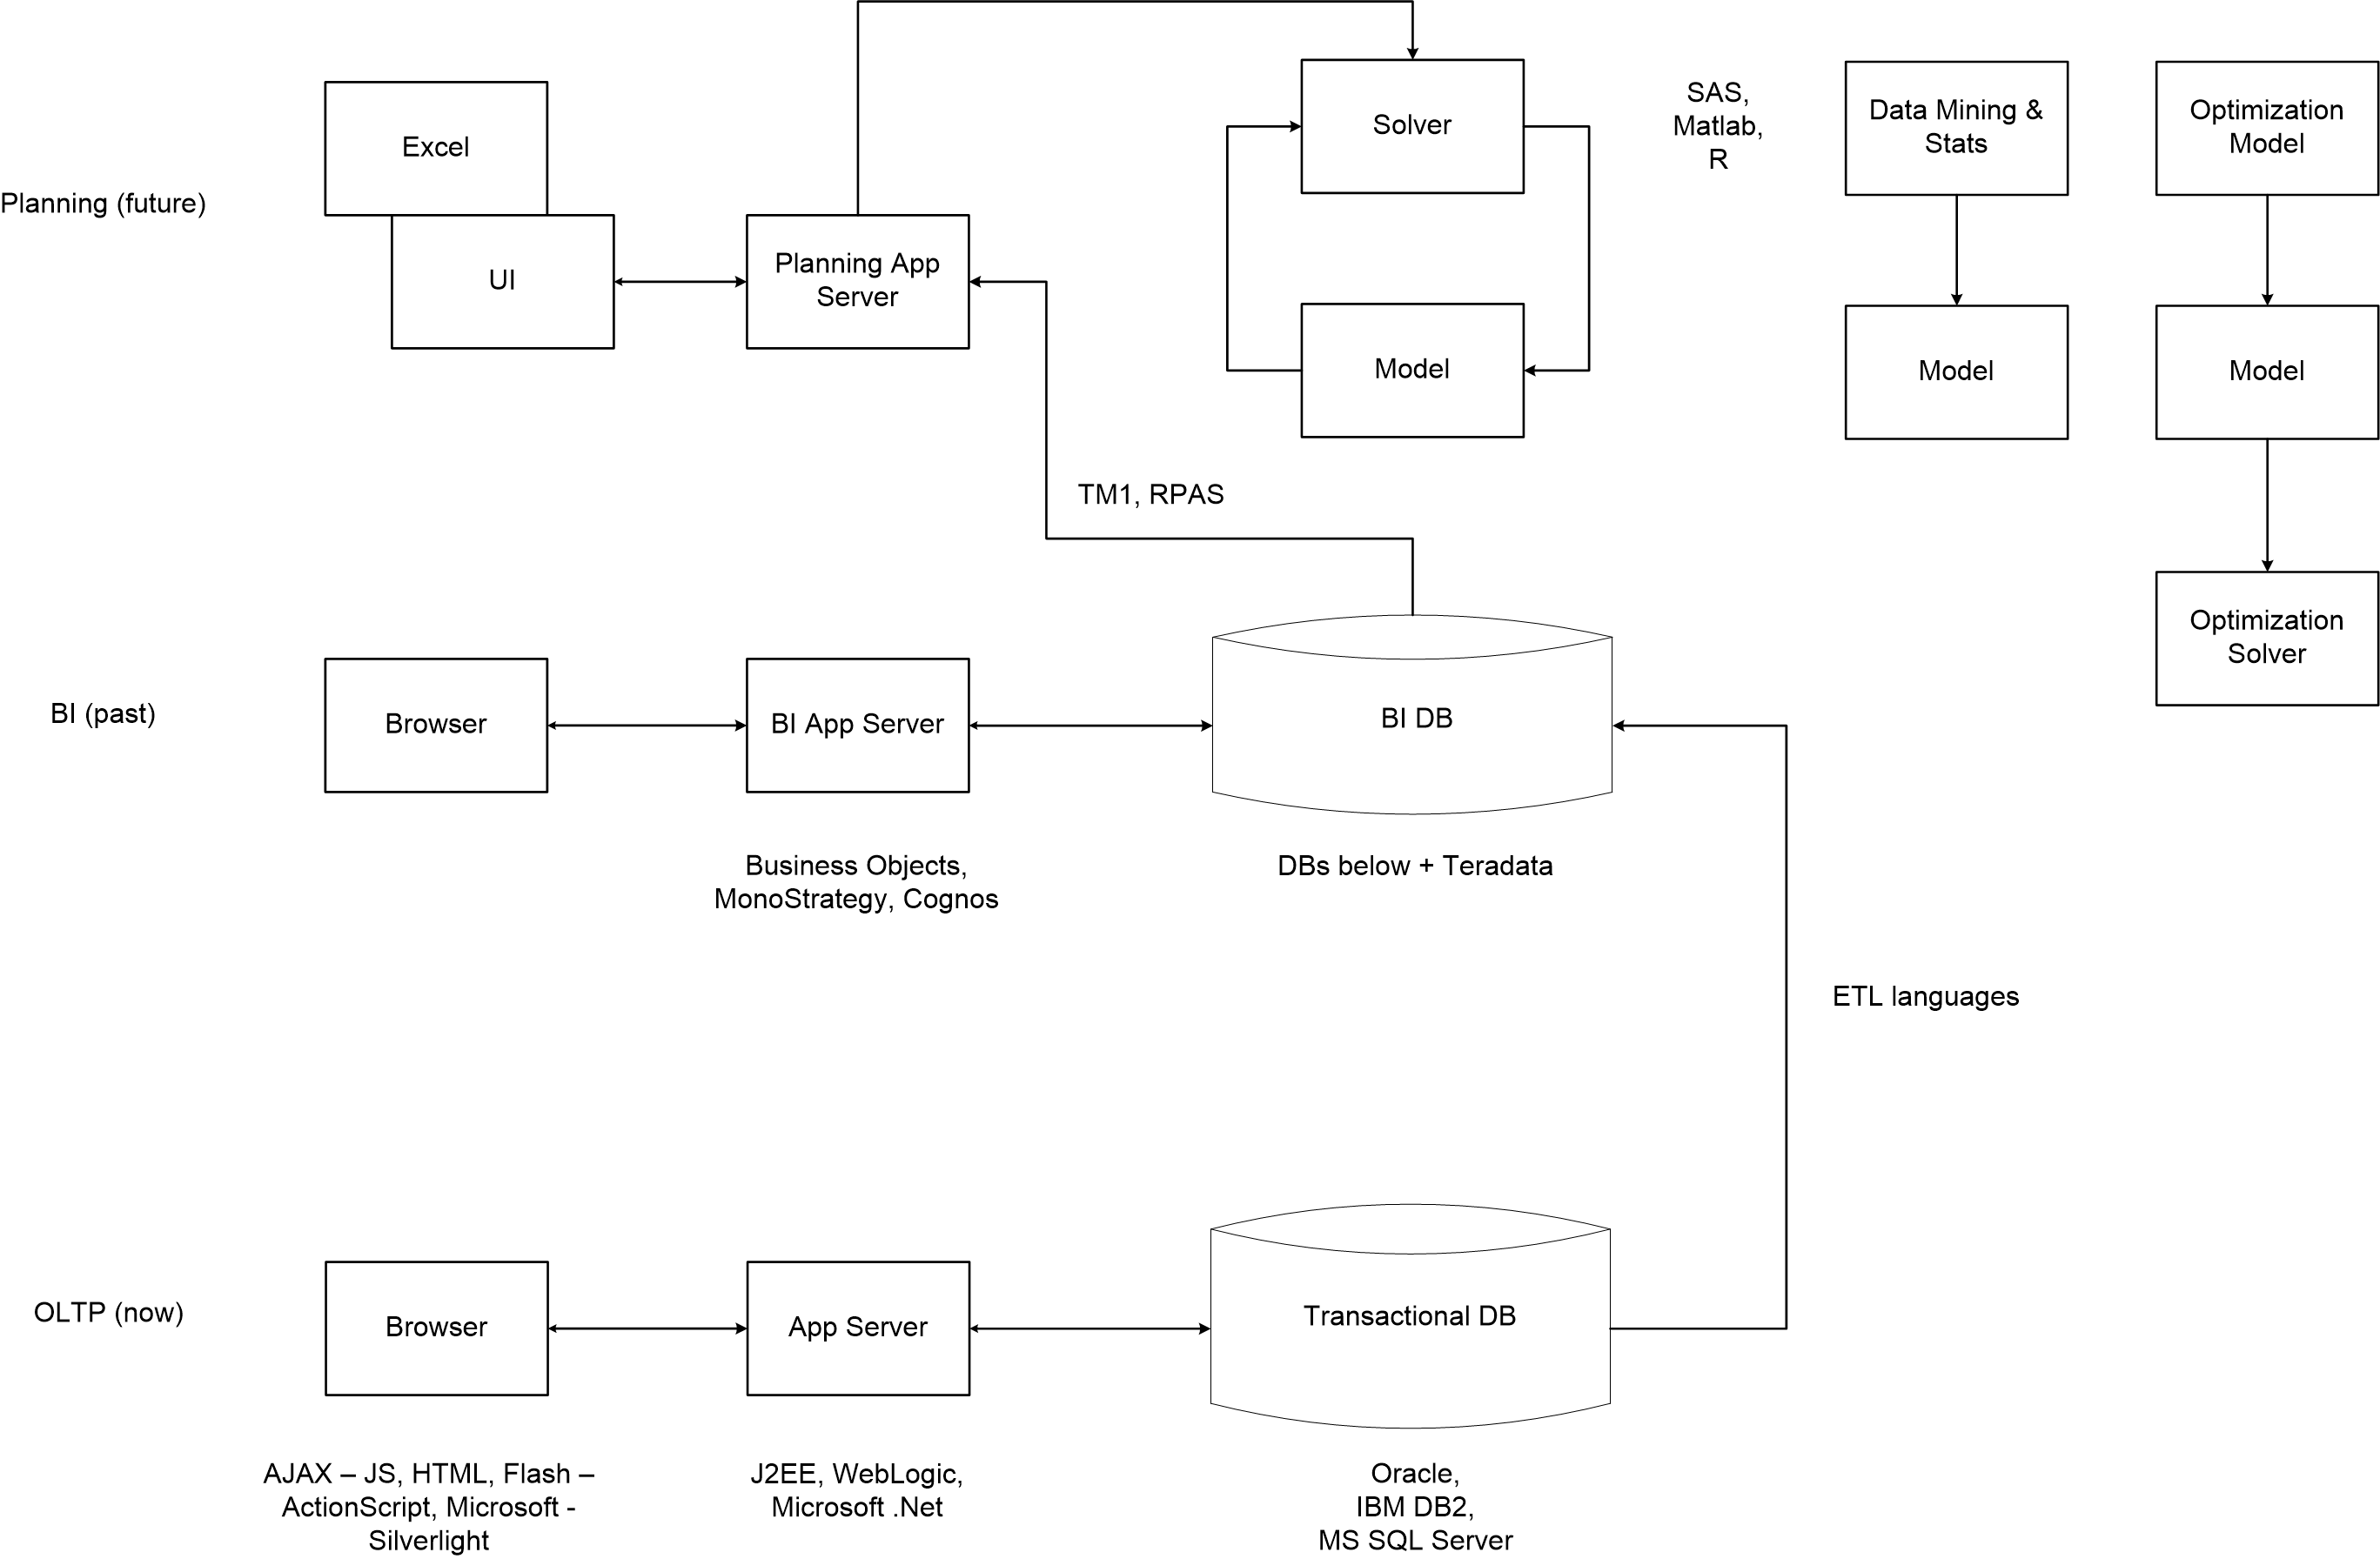
\includegraphics[scale=0.2]{apps.png}
	\caption{Структурная схема стандартного построения приложений}
	\label{fig:domain:standard_app:app_scheme}
\end{figure}

На рисунке \ref{fig:domain:standard_app:app_scheme} приведен пример схемы типичного построения приложений. Если посмотреть на всю построенную в итоге систему, которая выполняет нужные задачи ​− строит модели, поддерживает их ​− то можно увидеть, что результатом является достаточно запутанная «агломерация» используемых технологий. Это одна из причин, почему данная сфера пока что не вышла на высокие позиции.

В нижнем слое можно видеть то, что происходит в конкретный момент времени: что продается, сколько продается, текущее состояние продаж, запаса и т.п. Этот слой обычно разрабатывается с помощью достаточно обширного стека технологий ​− здесь можно увидеть и \oracle, и MS SQL, в сервере приложений это могут быть как \dotnet, так и J2EE, в \ui (браузер), как правило, \js.

Если же задача усложняется и на первый план выходит анализ данных, требование понимания пройденных этапов, то потребуется другой список используемых технологий. Здесь вместо транзакционных баз данных применяются BI базы. Имеется свой BI App Server, которые может решать требуемые задачи в направлении анализа данных.

Наконец, при наличии таких задач, как планирование, прогноз, расчет полученных в будущем значений, картинка превращается в верхний слой, на котором может использоваться машинное обучение, другие структуры анализа.

Понятно, что структура усложняется с каждым новым слоем, с каждым добавленным модулем системы. Это ведет к тому, что для реализации такой структуры необходимы группы специалистов в разных отраслях, для каждого компонента отдельно. Переходы между этими слоями возможны благодаря ETL языкам (\emph{Extract}, \emph{Transform}, \emph{Load}). Они включают в себя разного рода скрипты, «батники», которые перекидывают информацию туда и обратно. Это содержит и свои минусы, поскольку появляется временная зависимость при выполнении таких операций ​− это может достигать тех случаев, когда на анализ приходят устаревшие данные, потому что информация на текущий момент обновляется достаточно быстро.

Эксперты называют такую ситуация \emph{«hairball»} (клубок), который точно отражает данную ситуацию. Приведя в порядок отрицательные стороны такого приложения, можно выделить следующие пункты:
\begin{itemize}
  \item сложно разрабатывать приложения с большой вариацией языков и технологий ​− нужно большое количество инженеров и менеджеров для управления и координацией компонентов;
  \item разделение по слоям приводит к тому, что необходимы дополнительные затраты на передвижение данных между слоями ​− дорого и затратно по времени;
  \item сложность для пользователя в итоговой работе.
\end{itemize}

\subsection{Ключевые идеи платформы LogicBlox}
\label{sec:domain:framework_key_ideas}

База данных LogicBlox позволяет избавить от всей этой запутанности и сложности управления, поскольку внутри себя она содержит необходимые функции. Ее также называют «smart database» \cite{kurt_lecture}. Что же в данном контексте имеется в виду под словом smart?

Проведем аналогию со словом smartphone. Его основная цель ​− совершать звонки и отвечать на них. Кроме того, он позволяет нам делать фотографии, снимать видео, использовать GPS, будильник, часы и многое другое. Что его делает успешным в своем роде, так это то, что, возможно, он не делает профессиональную фотосъемку, как многие фотоаппараты, он не воспроизведет музыку со всеми тонкостями, но вместе с тем в нем собраны различные технологии, выполняющие различные функции и работающие на одной платформе . Поэтому ключевыми идеями создания платформы LogicBlox в целом являются:
\begin{enumerate}
  \item В ней самой выполняется большинство необходимых вычислений с данными, которые она содержит.
  \item Программирование выполняется с помощью декларативного языка программирования \logiql. Он предельно мощный для того, чтобы управлять большинством операций в текущем моделировании.
\end{enumerate}

Ключевые аспекты платформы:
\begin{itemize}
  \item объединение баз данных;
    \begin{enumerate}[leftmargin=5.5mm]
      \item вместо \olap и \oltp применяется подход HTAP (Hybrid Analytical Transactional Processing);
      \item выполнение математических и графовых оптимизаций, машинного обучения в самой базе;
      \item больше акцент на формирование бизнес-моделей, чем на ETL;
    \end{enumerate}
  \item объединение базы данных и большей части сервера приложений;
  \begin{enumerate}[leftmargin=5.5mm]
    \item единая декларативная модель для бизнес-логики и обработки данных;
    \item декларативные программируемые модель и язык;
  \end{enumerate}
\end{itemize}

% \begin{table}[ht]
% \caption{Категоризация архитектурных стилей}
% \label{table:analysis:architectures:categorization}
% \centering
%   \begin{tabular}{|>{\raggedright}m{0.27\textwidth}
%                   |>{\raggedright\arraybackslash}m{0.675\textwidth}|}
%   \hline Категория & Архитектурный стиль \\
%   \hline Связь & SOA (Service-oriented architecture -- архитектура, ориентированная на сервисы), Шина сообщений \\
%   \hline Развертывание & Клиент-серверный, трехуровневый, N-уровневый \\
%   \hline Предметная область & DDD (Domain-driven design -- проблемно-ориентированное проектирование) \\
%   \hline Структура & Компонентный, объектно-ориентированный, многоуровневый\\
%   \hline
%   \end{tabular}
% \end{table}

% \emph{Проблемно-ориентированный архитектурный стиль} основывается на\linebreakпредметной области, ее элементах, их поведении и связях между ними.

% \subsubsection{} Проектирование баз данных
% \label{sec:analysis:literature:db}
